% fig1_system_architecture.tex -- clean journal-style redraw
\documentclass[tikz,border=8pt]{standalone}
\usepackage{amsmath}
\renewcommand{\familydefault}{\sfdefault}
\usepackage{tikz}
\usetikzlibrary{arrows.meta,positioning,fit,calc}

\definecolor{analogBlue}{HTML}{2F5D8C}
\definecolor{analogFill}{HTML}{E7F0FA}
\definecolor{digitalOrange}{HTML}{C76B1E}
\definecolor{digitalFill}{HTML}{FFF0DF}
\definecolor{deviceGreen}{HTML}{2E7D5B}
\definecolor{deviceFill}{HTML}{E7F4EE}
\definecolor{noiseRed}{HTML}{B94A48}
\definecolor{ink}{HTML}{202020}
\definecolor{muted}{HTML}{666666}

\begin{document}
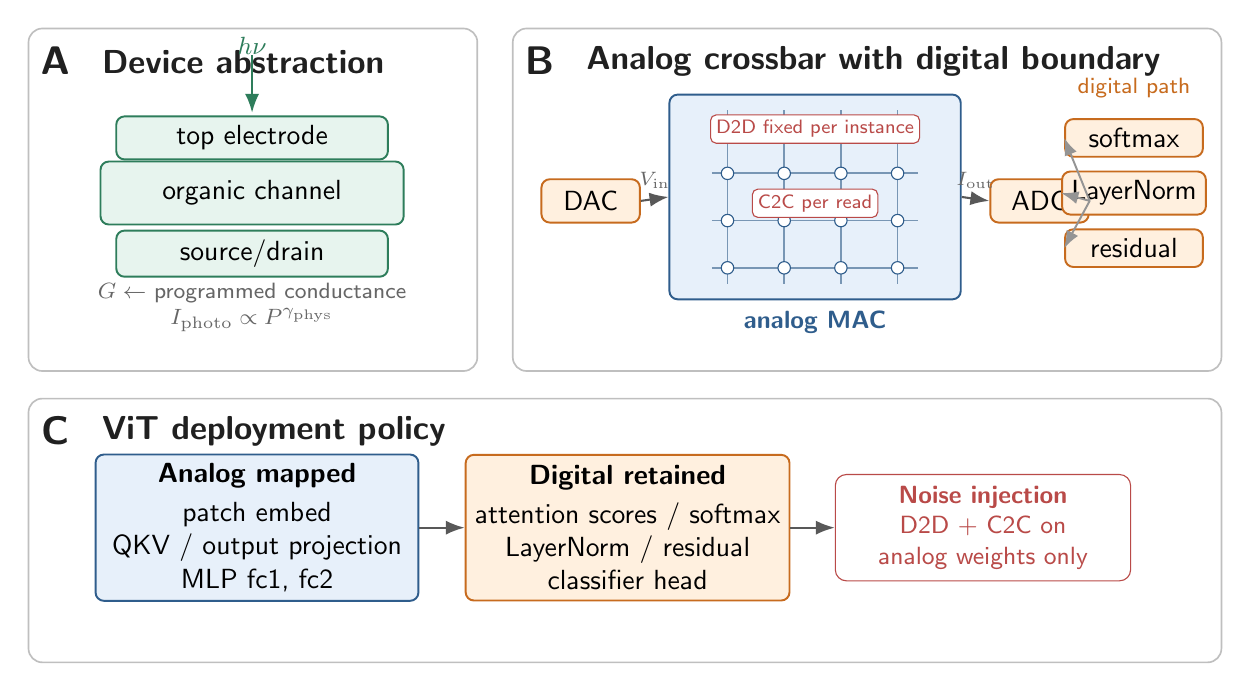
\begin{tikzpicture}[
  font=\sffamily,
  panel/.style={draw=black!25, rounded corners=5pt, fill=white, line width=0.6pt},
  title/.style={font=\sffamily\bfseries\large, text=ink, anchor=west},
  tag/.style={font=\sffamily\bfseries\Large, text=ink},
  small/.style={font=\sffamily\footnotesize, text=muted},
  tinylabel/.style={font=\sffamily\scriptsize, text=muted},
  analog/.style={draw=analogBlue, fill=analogFill, rounded corners=3pt, line width=0.7pt, align=center},
  digital/.style={draw=digitalOrange, fill=digitalFill, rounded corners=3pt, line width=0.7pt, align=center},
  device/.style={draw=deviceGreen, fill=deviceFill, rounded corners=3pt, line width=0.7pt, align=center},
  arrow/.style={-{Latex[length=2.4mm]}, line width=0.75pt, draw=ink!75},
  softarrow/.style={-{Latex[length=2.2mm]}, line width=0.7pt, draw=muted!70}
]

% ------------------------------------------------------------------
% Panel A: device abstraction
% ------------------------------------------------------------------
\node[panel, minimum width=5.7cm, minimum height=4.35cm, anchor=north west] (pa) at (0,4.35) {};
\node[tag] at ($(pa.north west)+(0.35,-0.42)$) {A};
\node[title] at ($(pa.north west)+(0.82,-0.43)$) {Device abstraction};

\node[device, minimum width=3.45cm, minimum height=0.42cm] (top) at (2.85,2.95) {top electrode};
\node[device, minimum width=3.85cm, minimum height=0.80cm] (semi) at (2.85,2.25) {organic channel};
\node[device, minimum width=3.45cm, minimum height=0.42cm] (bot) at (2.85,1.48) {source/drain};
\draw[arrow, deviceGreen] (2.85,4.0) -- (2.85,3.27);
\node[font=\sffamily\small, text=deviceGreen] at (2.85,4.12) {$h\nu$};
\node[small, align=center] at (2.85,0.80) {$G \leftarrow$ programmed conductance\\$I_{\mathrm{photo}} \propto P^{\gamma_{\mathrm{phys}}}$};

% ------------------------------------------------------------------
% Panel B: array + mixed-signal boundary
% ------------------------------------------------------------------
\node[panel, minimum width=9.0cm, minimum height=4.35cm, anchor=north west] (pb) at (6.15,4.35) {};
\node[tag] at ($(pb.north west)+(0.35,-0.42)$) {B};
\node[title] at ($(pb.north west)+(0.82,-0.43)$) {Analog crossbar with digital boundary};

\node[digital, minimum width=1.25cm, minimum height=0.55cm] (dac) at (7.15,2.15) {DAC};
\node[analog, minimum width=3.7cm, minimum height=2.6cm] (xb) at (10.0,2.2) {};
\node[digital, minimum width=1.25cm, minimum height=0.55cm] (adc) at (12.85,2.15) {ADC};
\draw[arrow] (dac.east) -- (xb.west) node[midway, above, tinylabel] {$V_{\mathrm{in}}$};
\draw[arrow] (xb.east) -- (adc.west) node[midway, above, tinylabel] {$I_{\mathrm{out}}$};

% Crossbar grid inside xb
\foreach \i in {0,...,3} {
  \draw[analogBlue!65, line width=0.65pt] ($(xb.west)+(0.55,0.9-0.6*\i)$) -- ($(xb.east)+(-0.55,0.9-0.6*\i)$);
  \draw[analogBlue!65, line width=0.65pt] ($(xb.west)+(0.75+0.72*\i,1.1)$) -- ($(xb.west)+(0.75+0.72*\i,-1.1)$);
}
\foreach \i in {0,...,3} {
  \foreach \j in {0,...,3} {
    \node[circle, draw=analogBlue, fill=white, minimum size=4.5pt, inner sep=0pt] at ($(xb.west)+(0.75+0.72*\j,0.9-0.6*\i)$) {};
  }
}
\node[font=\sffamily\small\bfseries, text=analogBlue] at ($(xb.south)+(0,-0.28)$) {analog MAC};
\node[draw=noiseRed, fill=white, rounded corners=2pt, inner sep=2pt, font=\sffamily\scriptsize, text=noiseRed] at ($(xb.north)+(0,-0.45)$) {D2D fixed per instance};
\node[draw=noiseRed, fill=white, rounded corners=2pt, inner sep=2pt, font=\sffamily\scriptsize, text=noiseRed] at ($(xb.center)+(0,-0.08)$) {C2C per read};

\node[digital, minimum width=1.75cm, minimum height=0.46cm] (soft) at (14.05,2.95) {softmax};
\node[digital, minimum width=1.75cm, minimum height=0.46cm] (norm) at (14.05,2.25) {LayerNorm};
\node[digital, minimum width=1.75cm, minimum height=0.46cm] (res) at (14.05,1.55) {residual};
\draw[softarrow] (adc.east) -- (soft.west);
\draw[softarrow] (adc.east) -- (norm.west);
\draw[softarrow] (adc.east) -- (res.west);
\node[small, text=digitalOrange] at (14.05,3.58) {digital path};

% ------------------------------------------------------------------
% Panel C: deployment policy
% ------------------------------------------------------------------
\node[panel, minimum width=15.15cm, minimum height=3.35cm, anchor=north west] (pc) at (0, -0.35) {};
\node[tag] at ($(pc.north west)+(0.35,-0.42)$) {C};
\node[title] at ($(pc.north west)+(0.82,-0.43)$) {ViT deployment policy};

\node[analog, minimum width=4.1cm, minimum height=1.85cm, anchor=west] (ana) at (0.85,-2.0)
{\textbf{Analog mapped}\\[2pt] patch embed\\QKV / output projection\\MLP fc1, fc2};
\node[digital, minimum width=4.1cm, minimum height=1.85cm, anchor=west] (dig) at (5.55,-2.0)
{\textbf{Digital retained}\\[2pt] attention scores / softmax\\LayerNorm / residual\\classifier head};
\node[draw=noiseRed, fill=white, rounded corners=4pt, minimum width=3.75cm, minimum height=1.35cm, align=center, font=\sffamily\small, text=noiseRed, anchor=west] (noise) at (10.25,-2.0)
{\textbf{Noise injection}\\D2D $+$ C2C on\\analog weights only};
\draw[arrow] (ana.east) -- (dig.west);
\draw[arrow] (dig.east) -- (noise.west);

\end{tikzpicture}
\end{document}
